\documentclass[10pt,a4paper]{article}
\usepackage[latin1]{inputenc}
\usepackage{graphicx,epsfig,palatino}
\usepackage[reqno,centertags]{amsmath}
\usepackage{tikz}
\usepackage{pgfplots}  
\usepackage{fancybox}
\usepackage{amsmath}
\usepackage[margin=1in]{geometry}
\setlength{\parindent}{0pt}
\setlength{\parskip}{4mm}
\graphicspath{{./figures/}}
\newcommand{\figuretikz}[3]{\pgfplotsset{width=#1\columnwidth,height=#1\columnwidth,compat=newest,plot coordinates/math parser=false}\input{#1}}
\newcommand{\tm}{\texttrademark}
\newcommand{\minbox}{\fbox{\rule{2mm}{0mm} \rule{0mm}{2mm}} }
\flushbottom

%%%%% My packages
\usepackage{listings}
\usepackage{amstext}
\usepackage{color, xcolor}
\usepackage{diagbox, tabularx}
%\usepackage{amsmath,mathtools,amssymb,amsfonts,dsfont,cancel} %Math Package
%%%%%

% MATLAB code settings
\lstset{extendedchars=false, % Shutdown no-ASCII compatible
basicstyle=\normalsize\tt, % the size of the fonts that are used for the code
language=Matlab, tabsize=4, numbers=left, numberstyle=\small, stepnumber=1, numbersep=8pt, keywordstyle=\color[rgb]{0,0,1}, commentstyle=\color[rgb]{0.133,0.545,0.133}, stringstyle=\color[rgb]{0.627,0.126,0.941}, backgroundcolor=\color{white}, showspaces=false, showstringspaces=false, showtabs=false, frame=single, captionpos=t, breaklines=true, breakatwhitespace=false, morekeywords={break, case, catch, continue, elseif, else, end, for, function, global, if, otherwise, persistent, return, switch, try, while}, title=\lstname,
mathescape=true,escapechar=? % escape to latex with ?..?  
escapeinside={\%*}{*)}, % if you want to add a comment within your code  
%morestring=[m]', % strings
%columns=fixed, % nice spacing
}

\begin{document}
\begin{titlepage}
%%%%%%%%%%%%%%%%%WRITE NAMES AND PERSONAL IDENTITY NUMBERS WHERE SPECIFIED IN FILE grade_template_to_include_eng.tex%%%%%%%%%%
\thispagestyle{empty}

\section*{\centerline{Grading template for laboratory exercise 3}\\
 \centerline{EL2820, Modeling of Dynamical Systems}
 \centerline{August 2018}}
\begin{center}
\vspace{-0.7cm}
  \small
%%%%%%%%%%%%%%%%%WRITE NAMES AND PERSONAL IDENTITY NUMBERS WHERE SPECIFIED%%%%%%%%%%
  \fbox{\parbox{0.95\columnwidth}{
      \begin{tabular}{lp{9cm}}
        \rule{0mm}{8mm} Chang, Hongsheng\\
        \rule{0mm}{8mm} 951228-2451\\
        \rule{0mm}{8mm} Jiang, Sifan\\
        \rule{0mm}{8mm} 961220-8232\\
      \end{tabular}}}
%%%%%%%%%%%%%%%%%DO NOT EDIT BELOW THIS LINE%%%%%%%%%%%%%%%%%%%%%%%%%%%
\vspace{-0.7cm}
  \begin{tabular}{lcc|cc}
    &\multicolumn{2}{c}{\bf Pass} &\multicolumn{2}{c}{\bf Fail}\\

    \rule{5cm}{0mm}  && yes& no & \\
    The report is handed in on time? && \minbox  & \minbox & \\

    \rule{5cm}{0mm} && $\le 2$st& $>2$ & \\
    Number of authors && \minbox  & \minbox & \\

    \rule{5cm}{0mm}  && yes& no & \\
    Author names and personal identity number filled out? && \minbox  & \minbox & \\

    \rule{5cm}{0mm}  &yes& often & sometimes & no\\
    The report is well structured? The language is understandable?&\minbox  &\minbox &\minbox
    &\minbox\\

    \rule{5cm}{0mm}  &yes& often & sometimes & no\\
    The figures are clear? (Captions, high resolution, etc.) &\minbox  &\minbox &\minbox
    &\minbox\\

    \rule{5cm}{0mm}  && yes& no & \\
    The preparation task is solved and motivated? && \minbox  & \minbox & \\

  \rule{5cm}{0mm}  && yes& no & \\
    The working region is defined and motivated? && \minbox  & \minbox & \\

  \rule{5cm}{0mm}  && yes& no & \\
    The sampling time is defined and motivated? && \minbox  & \minbox & \\

  \rule{5cm}{0mm}  && yes& no & \\
    A detailed description of the input signal is given and the choice is motivated? && \minbox  & \minbox & \\

  \rule{5cm}{0mm}  && yes& no & \\
    The amount of data used for estimation and validation is specified? && \minbox  & \minbox & \\


    \rule{5cm}{0mm}  && yes& no & \\
    Models of more than one model structure have been estimated? && \minbox  & \minbox & \\

 \rule{5cm}{0mm}  && yes& no & \\
    The model order of each model is motivated? && \minbox  & \minbox & \\


    \rule{5cm}{0mm}  && yes& no & \\
    A ranking of the estimated models have been made? && \minbox  & \minbox & \\


    \rule{5cm}{0mm}  && yes& no & \\
    The ranking is well motivated according to the requirements?  && \minbox  & \minbox & \\


    \rule{0mm}{7mm}&&&&\\
    \rule{5cm}{0mm}  && {\bf Pass} & {\bf Fail} & \\
    {\bf First review}  & & \minbox & \minbox  & \multicolumn{1}{l}{Sign:}\\
    %\multicolumn{5}{c}{\dotfill}\\
    \multicolumn{3}{c}{\rule{0mm}{5mm}\dotfill}&\multicolumn{2}{|c}{\rule{0mm}{5mm}\dotfill}\\
    \rule{5cm}{0mm}\rule{0mm}{5mm}  && {\bf Pass} & {\bf Fail} & \\
    {\bf Second review} (if failed in the first review)& &\minbox &\minbox & \multicolumn{1}{l}{Sign:}
  \end{tabular}
\vfill
\vspace{0.6cm}
\small
{\bf Pass}\\
\fbox{
  \noindent
  Signature:\rule{30mm}{0mm} \rule{0mm}{10mm}}


\end{center}

%%%%%%%%%%%%%%%%%%%%%%%%%%%%%%%%%%%%%%%%
\end{titlepage}
\newpage
\pagestyle{plain}
%%%%%%%%%%%%%%%%%%%%%%%%%%%%%%%%%%%%%%%%
\section{Preparation task}
\begin{itemize}
    \item Derivation of a physical model of the magnetic levitator in state-space form:
    \par From figure in the lab description, we can get:
	\begin{align}
		m \ddot{z} &= \gamma \dot{z} + E_{r} - F_{ul} - mg \\
		m \ddot{y} &= \gamma \dot{y} - E_{a} + F_{lu} - mg
	\end{align}
	\par Repulsive magnet force is proportional to $m \vert y - z \vert^{-4}$, and here, constant $T$ is given to represent the proportion:
	\begin{align}
		F_{ul} &= F_{lu} = T m \frac{1}{(y - z)^{4}}
	\end{align}
	\par From exercise 2.5, the electromagnetic force can be obtained, where $K$ is a constant and $A$ is the area of the coil:
	\begin{align}
		B &= \mu_{0} \frac{N \gamma^{2} I(t)}{2 y^{3}} \\
		E &= \frac{1}{2} A \frac{B^{2}(t)}{\mu_{0}} \\
		E &= \frac{A N^{2} \mu_{0} \gamma^{4}}{8} \frac{I^{2}(t)}{y^{6}(t)} = K m \frac{I^{2}(t)}{y^{6}(t)} \\
		\text{So:} \quad E_{a} &= K m \frac{I^{2}(t)}{y^{6}(t)} \qquad E_{r} = K m \frac{I^{2}(t)}{z^{6}(t)}
	\end{align}
	\par Then we can obtain state space equations:
	\begin{align}
		\dot{a} &= \frac{\gamma}{m} \dot{z} + K \frac{I^{2}}{z^{6}} - T \frac{1}{(y - z)^{4}} - g \\
		\dot{b} &= \frac{\gamma}{m} \dot{y} + K \frac{I^{2}}{y^{6}} - T \frac{1}{(y - z)^{4}} - g \\
		\dot{z} &= a \\
		\dot{y} &= b
	\end{align}
	\item Suggestion for a suitable model order for a linear model:
	\par In stationarity, we have:
	\begin{align}
		x &= \begin{bmatrix} a \\ b \\ z \\ y \end{bmatrix} \qquad \dot{x} = \begin{bmatrix} \dot{a} \\ \dot{b} \\ \dot{z} \\ \dot{y} \end{bmatrix} = 0 = \begin{bmatrix} f_{1}(a, b, z, y, I_{0}) \\ \vdots \\ f_{4}(a, b, z, y, I_{0}) \end{bmatrix}
	\end{align}
	\par The linearized system is given by:
	\begin{align}
		\dot{\mathbf{X}} &= A \mathbf{X} + B I(t) \\
		\mathbf{Y} &= C \mathbf{X} + D\\
		A &= \left. \begin{bmatrix} \frac{\partial f_{1}}{\partial a} & \cdots & \frac{\partial f_{1}}{\partial y} \\ \vdots & \ddots & \vdots \\ \frac{\partial f_{4}}{\partial a} & \cdots & \frac{\partial f_{4}}{\partial y} \end{bmatrix} \right|_{a = a^{0}, b = b^{0}, z = z^{0}, y = y^{0}, I = I_{0}} = \begin{bmatrix} \frac{\gamma}{m} & 0 & - \frac{4 T}{(y^{0} - z^{0})^{5}} - \frac{6 K I^{2}}{{z^{0}}^{7}} & \frac{4 T}{(y^{0} - z^{0})^{5}} \\ 0 & \frac{\gamma}{m} & \frac{4 T}{(y^{0} - z^{0})^{5}} & - \frac{4 T}{(y^{0} - z^{0})^{5}} + \frac{6 K I^{2}}{{y^{0}}^{7}} \\ 1 & 0 & 0 & 0 \\ 0 & 1 & 0 & 0 \end{bmatrix} \\ 
		B &= \left. \begin{bmatrix} \frac{\partial f_{1}}{\partial I} \\ \vdots \\ \frac{\partial f_{4}}{\partial I} \end{bmatrix} \right|_{a = a^{0}, b = b^{0}, z = z^{0}, y = y^{0}, I = I_{0}} = \begin{bmatrix} \frac{2 K I}{{z^{0}}^{6}} \\ - \frac{2 K I}{{z^{0}}^{6}} \\ 0 \\ 0 \end{bmatrix} \\
		C &= \begin{bmatrix} 0 & 0 & 0 & 1 \end{bmatrix}^{T} \qquad D = \begin{bmatrix} 0 & 0 & 0 & 0 \end{bmatrix}^{T}
	\end{align}
	\par Then the transform function is given as, where $\mathbf{I}$ is the identity matrix and $N^{a}_{i}$ is a polynomial of $i$ degree with label $a$ on nominator:
	\begin{align}
		G(q) &= C^{T}(q \mathbf{I} - A)^{-1}B + D \\
		&= \frac{N^{a}_{3}(q)}{D^{a}_{4}(q)} + \frac{N^{b}_{0}(q)}{D^{b}_{4}(q)}
	\end{align}
	\par Approximating $G(q)$ with $D^{a}_{4}(q) = D^{b}_{4}(q)$, the trasfer function would be $G(q) = \frac{N_{3}(q)}{D_{4}(q)}$. Plus, since our sampling time would be $2ms$ and the delay time would be $9ms$ in our experiment, base on the equation $n_{k} = \lfloor\frac{\tau}{h}\rfloor + 1$ from the lecture slides, we get $n_{k} = 5$. In all, our suggestion of the model order for ARX model could be ARX(4 3 5). Then the ARMAX and BJ models can be modified accordingly.
    \item \textsc{Matlab} codes for the required functions are attached in the page ~\pageref{matlabCode}.
    \item Plot for the spectrum of the binary random signal for the required values of $\alpha$ is shown in Fig.~\ref{fig:binarySpectrum}.
	\begin{figure}[h]
		\footnotesize
		\centering 
		%\def\svgwidth{.8\columnwidth}
		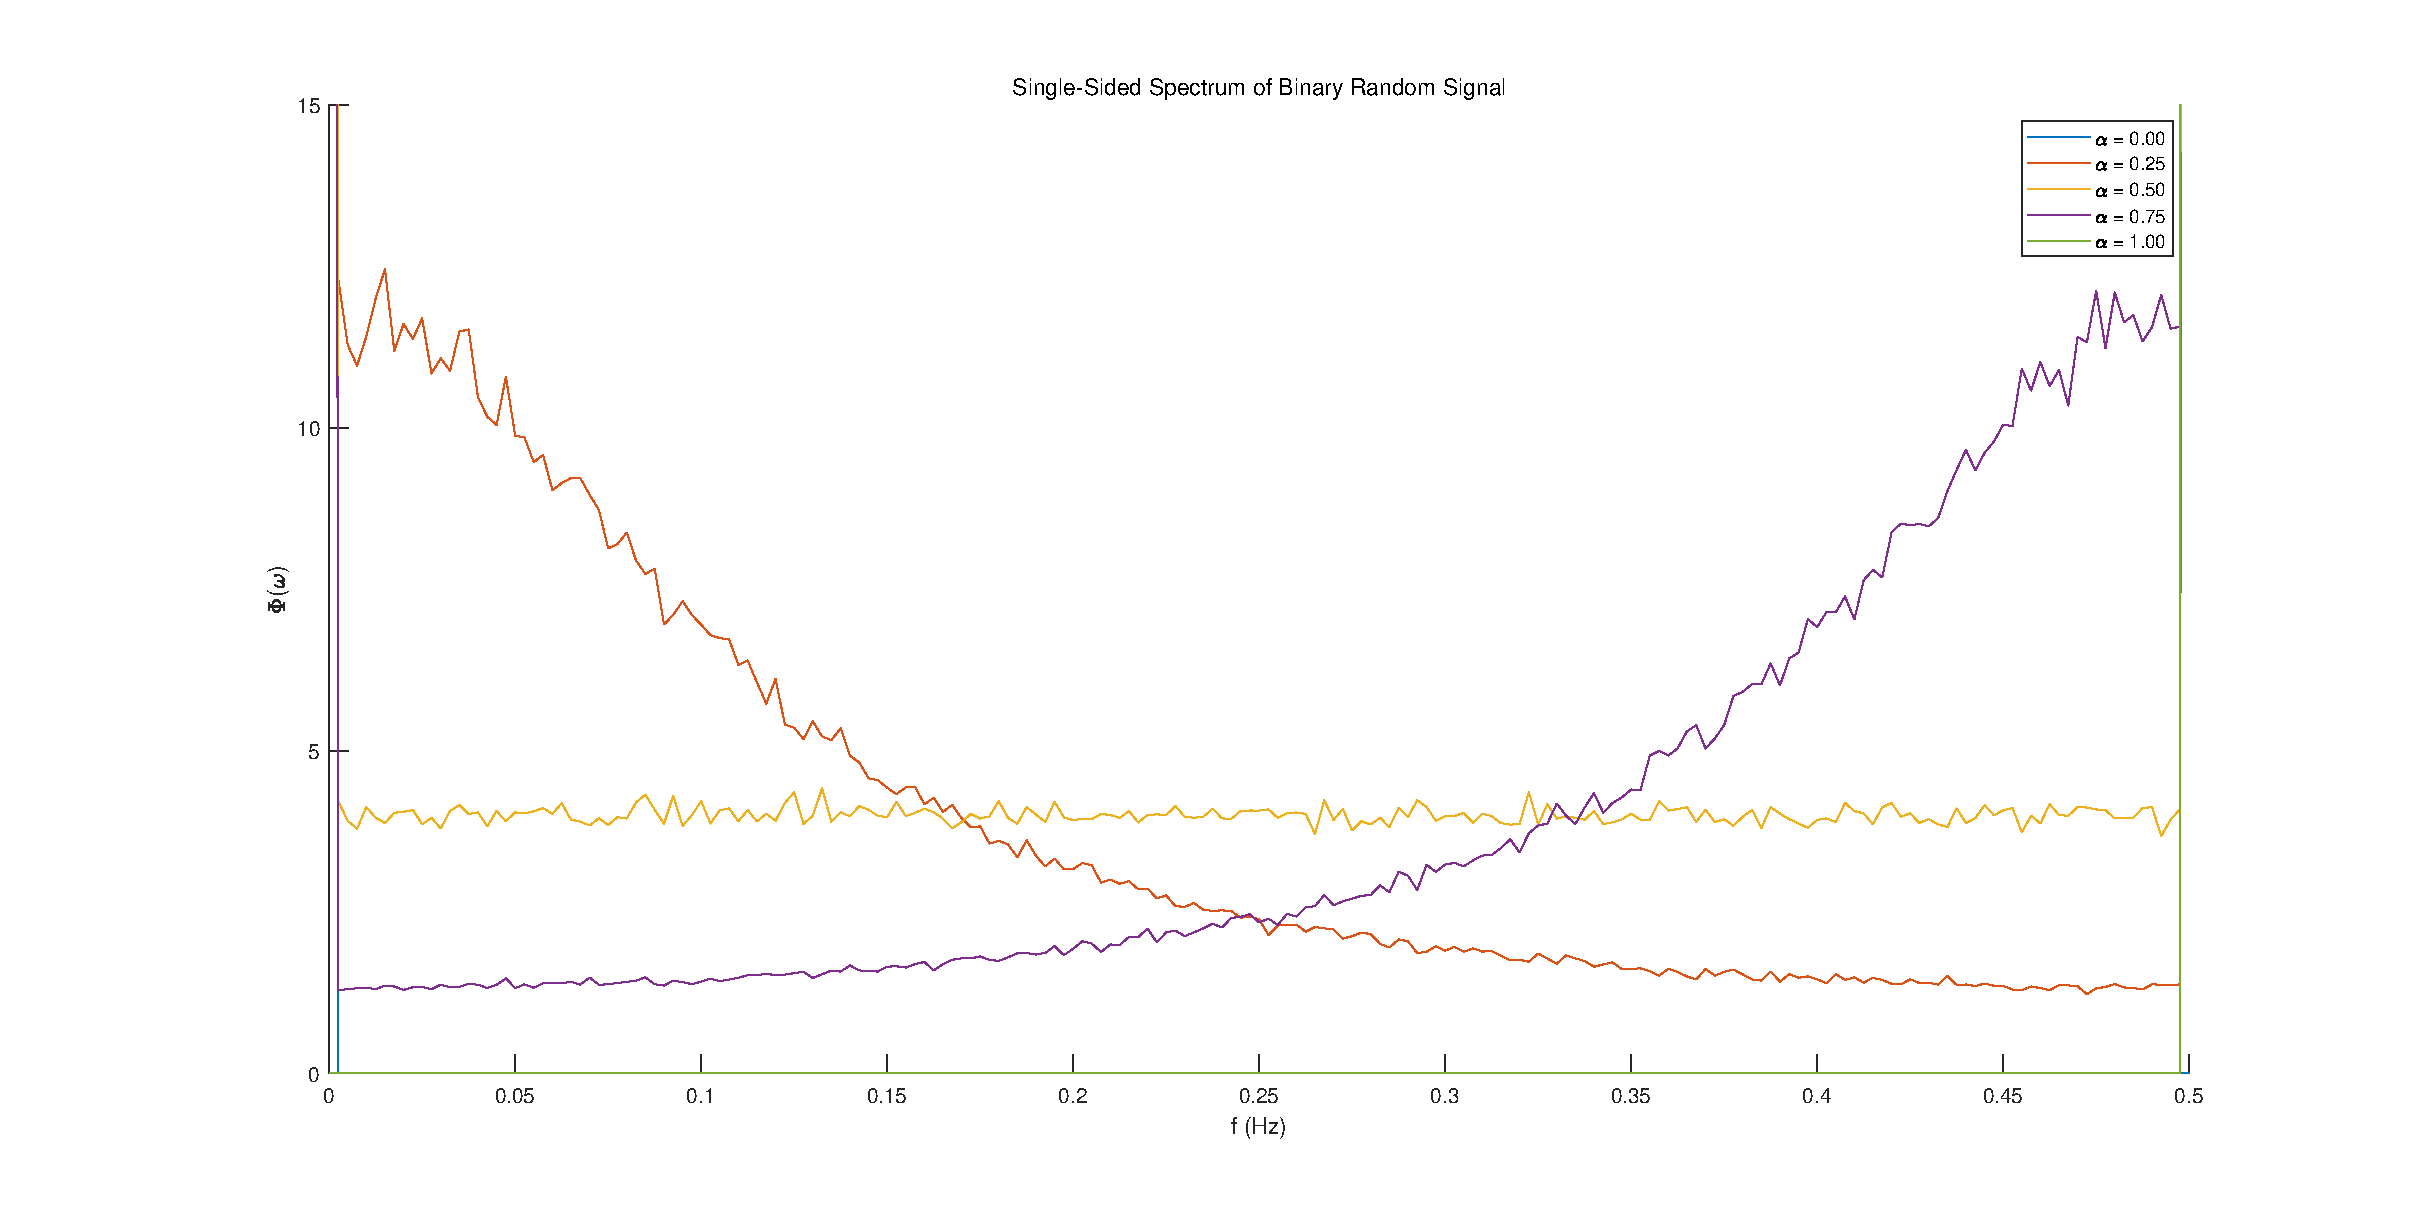
\includegraphics[width=0.7\columnwidth]{binarySpectrum.eps} 
		\caption{Spectrum of binary random signal.}
		\label{fig:binarySpectrum}
	\end{figure}
\end{itemize}
%%%%%%%%%%%%%%%%%%%%%%%%%%%%%%%%%%%%%%%%

%%%%%%%%%%%%%%%%%%%%%%%%%%%%%%%%%%%%%%%%
\section{Working region}
\begin{itemize}
    \item After the experiment, we choose working region as 1.5A $\sim$ 3.6A.
    \item Motivation for working region:
    \par From Fig.~\ref{fig:workingRegion}, we can see that when $u \in [1.5A, 3.6A]$, the plot have linearity.
    \item Plot for illustrating working region is shown in Fig.~\ref{fig:workingRegion}.
	\begin{figure}[h]
		\footnotesize
		\centering 
		%\def\svgwidth{.8\columnwidth}
		\includegraphics[width=0.7\columnwidth]{findWorkingRegion.png} 
		\caption{Working region.}
		\label{fig:workingRegion}
	\end{figure}
\end{itemize}
%	\begin{figure}[ht]
%		\footnotesize
%		\centering
%		\def\svgwidth{.8\columnwidth}
%		\input{figures/maglev_working.pdf_tex} 
%		\caption{Example of how to choose the working region.}
%		\label{fig:workingRegion}
%	\end{figure}
%%%%%%%%%%%%%%%%%%%%%%%%%%%%%%%%%%%%%%%%

%%%%%%%%%%%%%%%%%%%%%%%%%%%%%%%%%%%%%%%%
\section{Sampling time}
\begin{itemize}
    \item In the experiment, we chose $Ts = 2ms$ as sampling time.
    \item Motivation for sampling time:
    \par Fig.~\ref{fig:samplingTime} is obtained with the sampling time of $1ms$, and we can see the rise time is about $13ms$, which means there are about 13 points in one rise time. According to the requirement of ``the sampling time is set to give around four to ten samples per rise time'' in the lab description, we choose $2ms$ as sampling time so that there will be 6 to 7 samples per rise time.
    \item Plot of step responses yielding sampling time is shown in Fig.\ref{fig:samplingTime}.
    \begin{figure}[h]
		\footnotesize
		\centering 
		%\def\svgwidth{.8\columnwidth}
		\includegraphics[width=0.7\columnwidth]{findSamplingTime.png} 
		\caption{Step Response.}
		\label{fig:samplingTime}
	\end{figure}
\end{itemize}
%%%%%%%%%%%%%%%%%%%%%%%%%%%%%%%%%%%%%%%%
\begin{figure}[h]
		\footnotesize
		\centering
		%\def\svgwidth{.8\columnwidth}
		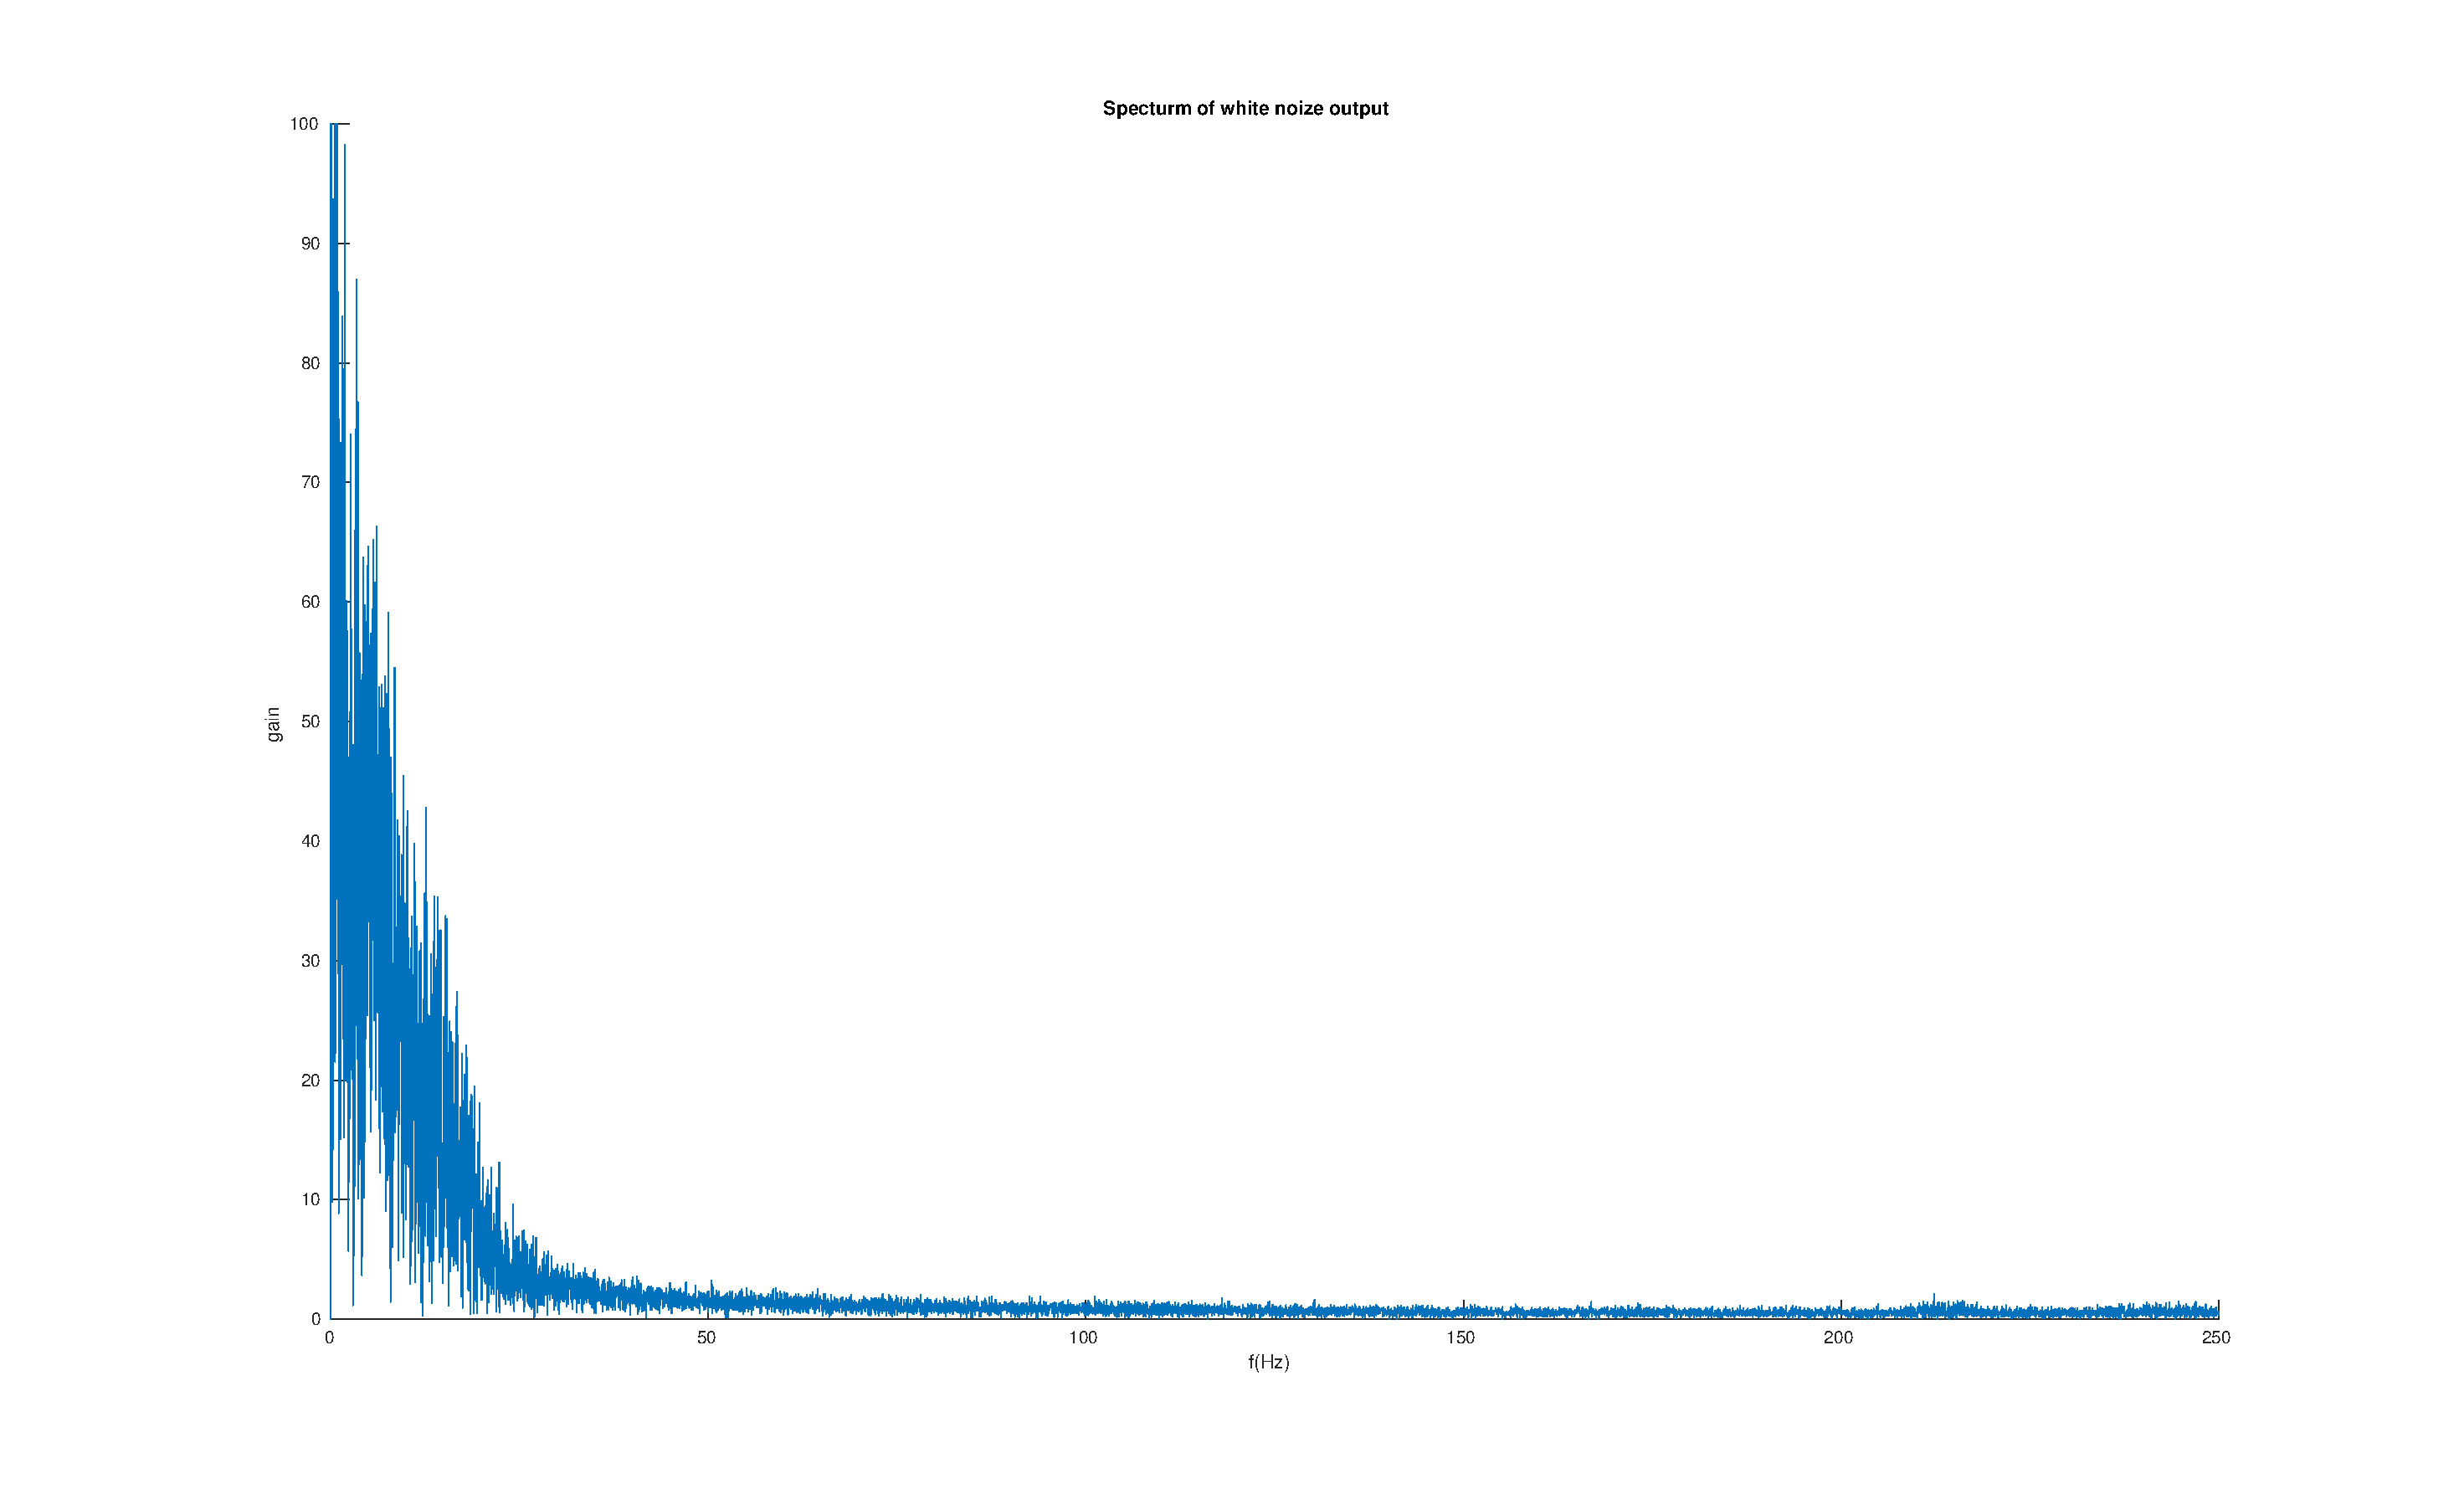
\includegraphics[width=0.7\columnwidth]{whiteNoiseSpectrum.eps} 
		\caption{Spectrum of white noise.}
		\label{fig:whiteNoiseSpectrum}
	\end{figure}
%%%%%%%%%%%%%%%%%%%%%%%%%%%%%%%%%%%%%%%%
\section{Input signals}
\begin{itemize}
    \item The binary random signal we choose have the similar output spectrum as the one of the white noises, which can be seen from Fig.~\ref{fig:binarySpectrum} and Fig.~\ref{fig:whiteNoiseSpectrum}.
    \item Motivation for chosen input signals:
    \par Comparing Fig.~\ref{fig:binarySpectrum} and Fig.~\ref{fig:whiteNoiseSpectrum}, when $\alpha=0.25$, the spectrum of binary random signal is simialr to the spectrum of white noise.
\end{itemize}
%%%%%%%%%%%%%%%%%%%%%%%%%%%%%%%%%%%%%%%%

%%%%%%%%%%%%%%%%%%%%%%%%%%%%%%%%%%%%%%%%
\section{Estimation and validation data}
\par Information about the amount of data used for identification and validation:
    \begin{table}[h]
	    \footnotesize
    	\centering
    	\caption{Data used for identification and validation.}
    	\label{table:data}
    	\begin{tabular}{lcccc}
    	\hline
    	Input signal & Value (A) & Amount of data & Estimation (s) & Validation (s) \\
    	\hline
    	Uniform white noise & [2, 3] & 10000 & [0, 10] & [10, 20] \\
    	Binary random signal with $\alpha = 0.25$ & [2, 3] & 10000 & [0, 10] & [10, 20] \\
    	\hline
    	\end{tabular}
    \end{table}
%%%%%%%%%%%%%%%%%%%%%%%%%%%%%%%%%%%%%%%%

%%%%%%%%%%%%%%%%%%%%%%%%%%%%%%%%%%%%%%%%
\section{Models}
\subsection{Model Description}
\begin{itemize}
	\item ARX model: $A(q) y[t] = B(q) u[k] + e[k]$, performs a filtering on both input and error with $\frac{1}{A}$ and adjust the transform function with B.
    \item ARMAX model: $A(q) y[t] = B(q) u[k] + C(q) e[k]$, is more generalized than ARX model with error being adjusted with C.
    \item BJ model: $y[k] = \frac{B(q)}{F(q)} u[k] + \frac{C(q)}{D(q)} e[k]$, includes all special cases.
\end{itemize}
\subsection{Motivation of Model Orders}
\begin{itemize}
\item ARX model: As mentioned in the ``Preparation task'' section, ARX(4 3 5) is first chosen for both white noise and binary random signal. In the case of white noise, it performs well enough. In the case of binary random signal, ARX(5 3 5) is chosen for obvious performance improvement.
\item ARMAX model: Based on ARX model, we try different values on $n_{c}$ and finally choose ARMAX(4 3 4 5) since performance drops when $n_{c} > 4$. For same reason, we choose ARMAX(5 3 2 5) for binary random signal.
\item BJ model: Based on ARMAX model, we get BJ(3 4 4 4 5) for white noise and BJ(3 2 5 5 5) for binary random signal since we don't need to change the order for each polynomial in each transform function.
\end{itemize}
\subsection{White Noise Signal Identification}

\subsubsection{Plots and Analysis} % Bode diagrams, poles and zeros.
\subsubsection{Validation and Correlation Analysis}
\subsection{Binary Random Signal Identification}
\subsubsection{Plots and Analysis} % Bode diagrams, poles and zeros.
\subsubsection{Validation and Correlation Analysis}
\subsection{Ranking and Comparison}
\begin{itemize}
   \item validation performed with simulation (\texttt{compare} with \texttt{M=inf}) and correlation analysis (\texttt{resid}).
   \item analysis/interpretations of validation and correlation analysis.
   \item a comparison between the accuracy of models obtained with different input signals (binary random signals v/s uniformly distributed white noise)
   \item A ranking of estimated models with respect to how well they describe the process, along with a rigorous motivation of chosen ranking. (Compare the analysis of plots, validation and correlation analysis for the different models.)
	\begin{table}[h]
		\footnotesize
		\centering
		\caption{Ranking of the Estimated Models with 1-step Prediction}
		\label{table:rank}
		\begin{tabular}{|l|lll|}
		\hline
		& \multicolumn{3}{c|}{Validation Data} \\
		\hline
		Rank & White Noise 1 & White Noise 2 & Binary Random Signal\\
		\hline
		1 & ARMAX(4 3 4 5) WH2: 89.33\% & BJ(3 4 4 4 5) WH1: 92.15\% & BJ(3 2 5 5 5) BR: 98.54\% \\
		2 & BJ(3 4 4 4 5) WH2: 89.11\% & ARMAX(4 3 4 5) WH1: 91.90\% & ARMAX(5 3 2 5) BR: 98.53\% \\
		3 & ARX(4 3 5) WH2: 88.91\% & BJ(3 4 4 4 5) WH2: 91.73\% & ARX(5 3 5) BR: 98.36\%\\
		4 & BJ(3 4 4 4 5) WH1: 88.80\% & ARMAX WH2: 91.71\% & ARMAX(4 3 4 5) WH1: 97.93\%\\
		\hline
		\end{tabular}
	\end{table}
\end{itemize}
%%%%%%%%%%%%%%%%%%%%%%%%%%%%%%%%%%%%%%%%

\newpage
%%%%%%%%%%%%%%%%%%%%%%%%%%%%%%%%%%%%%%%%
\section*{Attachments}
	\label{matlabCode}
    \lstinputlisting{generateBinarySignal.m}
	\lstinputlisting{getAverage.m}
	\lstinputlisting{getStationaryAverages.m}
	\lstinputlisting{findWorkingRegion.m}
%%%%%%%%%%%%%%%%%%%%%%%%%%%%%%%%%%%%%%%%
\end{document}
